%%% LaTeX Template: Article/Thesis/etc. with colored headings and special fonts
%%%
%%% Source: http://www.howtotex.com/
%%% Feel free to distribute this template, but please keep to referal to http://www.howtotex.com/ here.
%%% February 2011
%%%
%%% Modified January 2016 by CDM

%%%  Preamble
\documentclass[11pt,letterpaper]{article}
\usepackage[margin=1.0in]{geometry}
\usepackage[T1]{fontenc}
\usepackage[bitstream-charter]{mathdesign}
\usepackage[latin1]{inputenc}					
\usepackage{amsmath}						
\usepackage{xcolor}
\usepackage{cite}
\usepackage{hyphenat}
\usepackage{graphicx}
\usepackage{float}
\usepackage{subfigure}
\usepackage{sectsty}
\usepackage[compact]{titlesec} 
\usepackage[tablegrid]{vhistory}
\usepackage{pbox}
\allsectionsfont{\color{accentcolor}\scshape\selectfont}

%%% Definitions
\definecolor{accentcolor}{rgb}{0.0,0.0,0.5} 
\newcommand{\teamname}{Team Name}
\newcommand{\productname}{Product Name}
\newcommand{\coursename}{CSE 4316: Senior Design I}
\newcommand{\semester}{Fall 2015}
\newcommand{\docname}{Architectural Design Specification}
\newcommand{\department}{Department of Computer Science \& Engineering}
\newcommand{\university}{The University of Texas at Arlington}
\newcommand{\authors}{Alan Turing \\ Grace Hopper \\ John Von Neumann \\ Ada Lovelace \\ Charles Babbage}

%%% Headers and footers
\usepackage{fancyhdr}
	\pagestyle{fancy}						% Enabling the custom headers/footers
\usepackage{lastpage}	
	% Header (empty)
	\lhead{}
	\chead{}
	\rhead{}
	% Footer
	\lfoot{\footnotesize \teamname \ - \semester}
	\cfoot{}
	\rfoot{\footnotesize page \thepage\ of \pageref{LastPage}}	% "Page 1 of 2"
	\renewcommand{\headrulewidth}{0.0pt}
	\renewcommand{\footrulewidth}{0.4pt}

%%% Change the abstract environment
\usepackage[runin]{abstract}			% runin option for a run-in title
%\setlength\absleftindent{30pt}			% left margin
%\setlength\absrightindent{30pt}		% right margin
\abslabeldelim{\quad}	
\setlength{\abstitleskip}{-10pt}
\renewcommand{\abstractname}{}
\renewcommand{\abstracttextfont}{\color{accentcolor} \small \slshape}	% slanted text

%%% Start of the document
\begin{document}

%%% Cover sheet
{\centering \huge \color{accentcolor} \sc \textbf{\department \\ \university} \par}
\vspace{1 in}
{\centering \huge \color{accentcolor} \sc \textbf{\docname \\ \coursename \\ \semester} \par}
\vspace{0.5 in}
\begin{figure}[h!]
	\centering
   	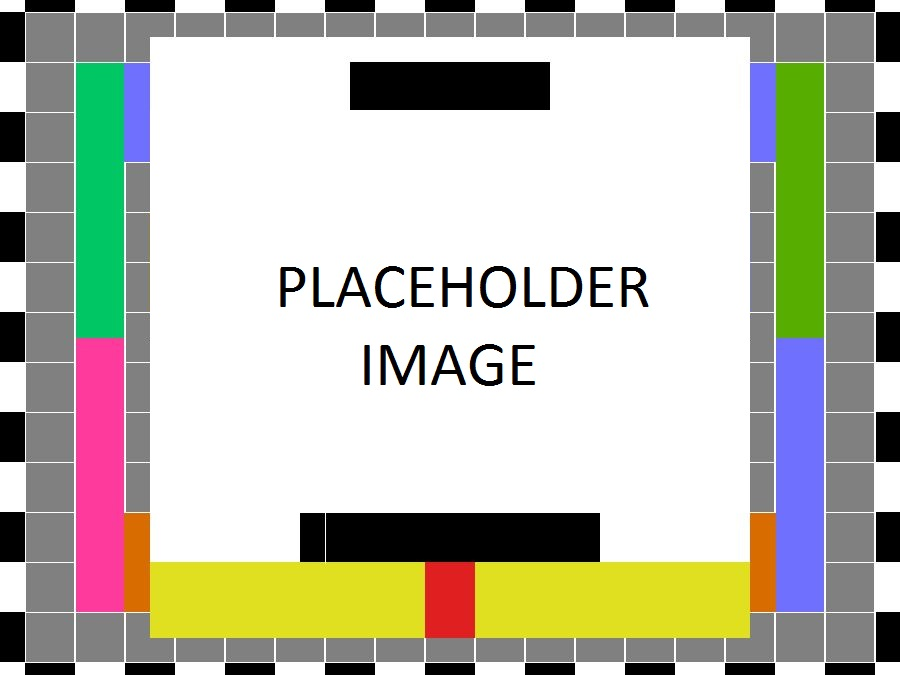
\includegraphics[width=0.60\textwidth]{images/test_image}
\end{figure}
\vspace{0.5 in}
{\centering \huge \color{accentcolor} \sc \textbf{\teamname \\ \productname} \par}
\vspace{0.5 in}
{\centering \large \sc \textbf{\authors} \par}
\newpage


%\vspace{1 in}
%\centerline{January 13th, 2012}
%\newpage

%%% Revision History
\begin{versionhistory}
  	\vhEntry{0.1}{10.01.2015}{GH}{document creation}
  	\vhEntry{0.2}{10.05.2015}{AT|GH}{complete draft}
  	\vhEntry{0.3}{10.12.2015}{AT|GH}{release candidate 1}
  	\vhEntry{1.0}{10.20.2015}{AT|GH|CB}{official release}
  	\vhEntry{1.1}{10.31.2015}{AL}{added design review requests}
\end{versionhistory}
\newpage

%%% Table of contents
\setcounter{tocdepth}{2}
\tableofcontents
\newpage

%%% List of figures and tables (optional)
\listoffigures
\listoftables
\newpage

%%% Document sections
\section{Introduction}
Your introduction should provide a brief overview of the product concept and a reference to the requirement specification and architectural design documents in 1 or 2 paragraphs. The purpose is to provide the reader with the location of relevant background material that lead to the design details presented in this document.

\newpage
\section{System Overview}
The overall structure of the software system is designed to seamlessly support the palletizing tasks of the UR20 robot arm system. This layered design enables modular functionality, enhancing system adapability and ensuring each layer performs a unique function while simultaneously providing crucial information to the main PLC layer which manages data distribution. As the central interface, the PLC efficiently processes the flow of sata from each subsystem layer, allowing for smooth system integration and effective coordination across all layers. This architecture promotes reliable, dynamic operation, optimizing the UR20's performance in real-time palletizing tasks.
\begin{figure}[h!]
	\centering
 	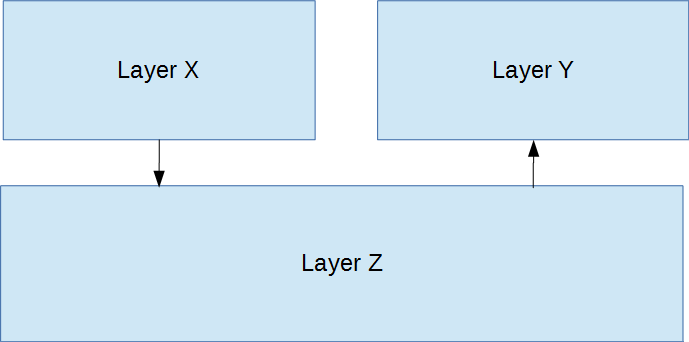
\includegraphics[width=0.60\textwidth]{images/layers}
 \caption{UR20 Architectural design diagram}
\end{figure}

\subsection{Layer 1: PLC Description}
The PLC will process most of the data through its peripherals, as seen in Figure 1. It is the primary interface between the different layers of the project. The built-in PLC will be configured with URScript, a Python-based scripting language in which vital functions will reside, such as the input function, the box offset algorithm, and finally, a position algorithm. The data flow will start with the input given by the QR code scanner or the safety sensor, and the input functions will follow these two data paths. First being, an input given by the QR code scanner will pass through the input function, which will then call the box offset algorithm to determine where the box is in 3D space given the location info from the QR code, which will go to the position algorithm which will determine the motion necessary for the UR20 to satisfy this request. The safety algorithm will give the second path, which will trigger the input function and call the position algorithm to safely slow down the speed at which the UR20 is palletizing to create a safe work area for a cooperative application.

\subsection{Layer 2: Safety Sensor}
The Safety Sensor will determine if a human is in the area of the UR20 arm. If so, it will reduce the speed of the UR20 in order to create a safe work environment. This will be achieved with the use of a camera that will process the data in real-time with the use of computer vision, which will send a signal to the PLC which in turn will send a signal to the UR20 movement subsystem in order to maintain a safe speed for collaborative work.

\subsection{Layer 3: UR20 Robot Arm}
UR20 Arm consists of a vacuum gripper, the gripper controller, and the movement of the arm. The arm is the physical output of the software that resides in the PLC layer. Additionally, it contains a gripper grab/release controller (the controller for the air compressor), which will be turned on or off when needed to hold or drop a box. The commands given by the PLC will determine the position and orientation needed for the UR20 to place the box correctly.

\subsection{Layer 4: QR Code Scanner}
Implementing QR code technology will enhance the automation and accuracy of arranging boxes on a pallet. When a box arrives on the conveyor belt, a QR code scanner positioned above the belt reads the QR code on the box. This QR code contains data such as box size, weight, and any other relevant handling instructions. Once scanned, the data is immediately sent to a Programmable Logic Controller (PLC) on a Universal Robots UR20 robotic arm system, which is responsible for arranging the boxes on the pallet.

\subsection{Layer 5: Conveyor Belt}
The conveyor belt system moves over pulleys driven by a motor. As the motor rotates, it propels the belt forward, allowing items placed on the belt to be conveyed along its length. The belt's speed can be adjusted to control the pace of movement. However, for this implementation, it will have two states: on or off. At the end of the conveyor belt, there will be a guide to reorient the boxes and a bracket in which the QR code scanner will be placed.
\newpage
\section{Subsystem Definitions \& Data Flow}

\begin{itemize}
    \item \textbf{Conveyor Belt Layer}
    \begin{itemize}
        \item ON/OFF Controller
    \end{itemize}

    \item \textbf{Safety Sensor Layer}
    \begin{itemize}
        \item Computer Vision
        \item UR20 Arm Speed Controller
    \end{itemize}

    \item \textbf{QR Layer}
    \begin{itemize}
        \item Scanner
        \item PLC Interface
    \end{itemize}

    \item \textbf{UR20 Robot Arm Layer}
    \begin{itemize}
        \item Vacuum Gripper
        \item Grab Release Control
        \item Movement
    \end{itemize}

    \item \textbf{PLC Layer}
    \begin{itemize}
        \item Input Function
        \item Box Offset Algorithm
        \item Position Algorithm
    \end{itemize}
\end{itemize}
\begin{figure}[h!]
	\centering
 	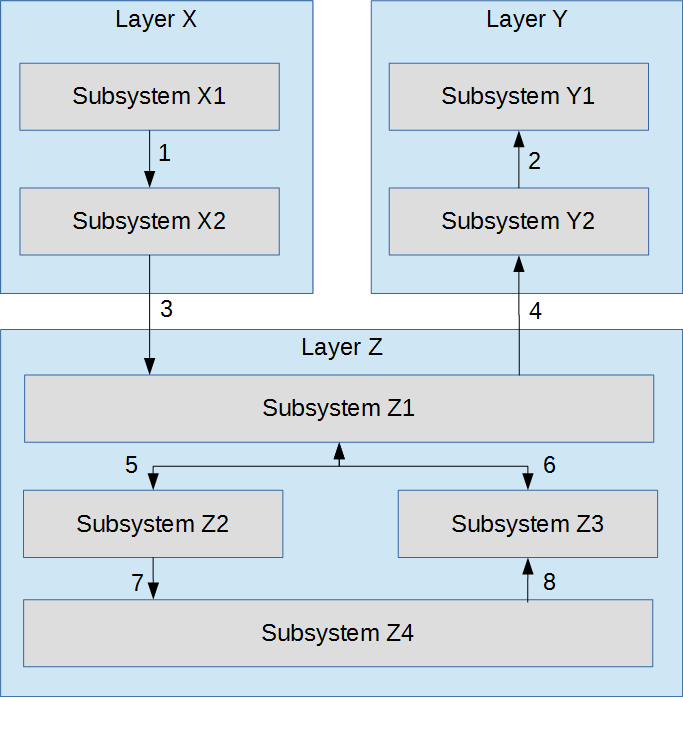
\includegraphics[width=\textwidth]{images/data_flow}
 \caption{UR20 Data flow diagram}
\end{figure}
\newpage
\section{X Layer Subsystems}
In this section, the layer is described in terms of the hardware and software design. Specific implementation details, such as hardware components, programming languages, software dependencies, operating systems, etc. should be discussed. Any unnecessary items can be ommitted (for example, a pure software module without any specific hardware should not include a hardware subsection). The organization, titles, and content of the sections below can be modified as necessary for the project.

\subsection{Layer Hardware}
A description of any involved hardware components for the layer. For example, if each subsystem is a software process running on an embedded computer, discuss the specifics of that device here. Do not list a hardware component that only exists at the subsystem level (include it in the following sections).

\subsection{Layer Operating System}
A description of any operating systems required by the layer.

\subsection{Layer Software Dependencies}
A description of any software dependencies (libraries, frameworks, etc) required by the layer.

\subsection{Subsystem 1}
Descibe at a high level the purpose and basic design of this subsystem. Is it a piece of hardware, a class, a web service, or something else? Note that each of the subsystem items below are meant to be specific to that subystem and not a repeat of anything discussed above for the overall layer.

\begin{figure}[h!]
	\centering
 	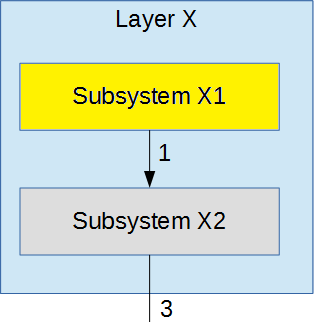
\includegraphics[width=0.60\textwidth]{images/subsystem}
 \caption{Example subsystem description diagram}
\end{figure}

\subsubsection{Subsystem Hardware}
A description of any involved hardware components for the subsystem.

\subsubsection{Subsystem Operating System}
A description of any operating systems required by the subsystem.

\subsubsection{Subsystem Software Dependencies}
A description of any software dependencies (libraries, frameworks, design software for mechanical parts or circuits, etc) required by the subsystem.

\subsubsection{Subsystem Programming Languages}
A description of any programming languages used by the subsystem.

\subsubsection{Subsystem Data Structures}
A description of any classes or other data structures that are worth discussing for the subsystem. For example, data being transmitted from a microcontroller to a PC via USB should be first be assembled into packets. What is the structure of the packets?

\subsubsection{Subsystem Data Processing}
A description of any algorithms or processing strategies that are worth discussing for the subsystem. If you are implementing a well-known algorithm, list it. If it is something unique to this project, discuss it in greater detail.



\newpage
\section{Y Layer Subsystems}
In this section, the layer is described in terms of the hardware and software design. Specific implementation details, such as hardware components, programming languages, software dependencies, operating systems, etc. should be discussed. Any unnecessary items can be ommitted (for example, a pure software module without any specific hardware should not include a hardware subsection). The organization, titles, and content of the sections below can be modified as necessary for the project.

\subsection{Layer Hardware}
A description of any involved hardware components for the layer. For example, if each subsystem is a software process running on an embedded computer, discuss the specifics of that device here. Do not list a hardware component that only exists at the subsystem level (include it in the following sections).

\subsection{Layer Operating System}
A description of any operating systems required by the layer.

\subsection{Layer Software Dependencies}
A description of any software dependencies (libraries, frameworks, etc) required by the layer.

\subsection{Subsystem 1}
Descibe at a high level the purpose and basic design of this subsystem. Is it a piece of hardware, a class, a web service, or something else? Note that each of the subsystem items below are meant to be specific to that subystem and not a repeat of anything discussed above for the overall layer.

\begin{figure}[h!]
	\centering
 	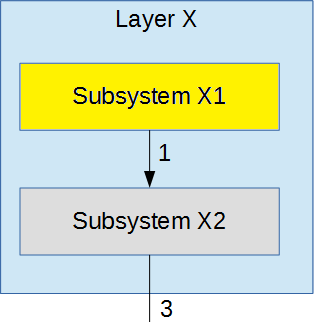
\includegraphics[width=0.60\textwidth]{images/subsystem}
 \caption{Example subsystem description diagram}
\end{figure}

\subsubsection{Subsystem Hardware}
A description of any involved hardware components for the subsystem.

\subsubsection{Subsystem Operating System}
A description of any operating systems required by the subsystem.

\subsubsection{Subsystem Software Dependencies}
A description of any software dependencies (libraries, frameworks, design software for mechanical parts or circuits, etc) required by the subsystem.

\subsubsection{Subsystem Programming Languages}
A description of any programming languages used by the subsystem.

\subsubsection{Subsystem Data Structures}
A description of any classes or other data structures that are worth discussing for the subsystem. For example, data being transmitted from a microcontroller to a PC via USB should be first be assembled into packets. What is the structure of the packets?

\subsubsection{Subsystem Data Processing}
A description of any algorithms or processing strategies that are worth discussing for the subsystem. If you are implementing a well-known algorithm, list it. If it is something unique to this project, discuss it in greater detail.



\newpage
\section{Z Layer Subsystems}
In this section, the layer is described in terms of the hardware and software design. Specific implementation details, such as hardware components, programming languages, software dependencies, operating systems, etc. should be discussed. Any unnecessary items can be ommitted (for example, a pure software module without any specific hardware should not include a hardware subsection). The organization, titles, and content of the sections below can be modified as necessary for the project.

\subsection{Layer Hardware}
A description of any involved hardware components for the layer. For example, if each subsystem is a software process running on an embedded computer, discuss the specifics of that device here. Do not list a hardware component that only exists at the subsystem level (include it in the following sections).

\subsection{Layer Operating System}
A description of any operating systems required by the layer.

\subsection{Layer Software Dependencies}
A description of any software dependencies (libraries, frameworks, etc) required by the layer.

\subsection{Subsystem 1}
Descibe at a high level the purpose and basic design of this subsystem. Is it a piece of hardware, a class, a web service, or something else? Note that each of the subsystem items below are meant to be specific to that subystem and not a repeat of anything discussed above for the overall layer.

\begin{figure}[h!]
	\centering
 	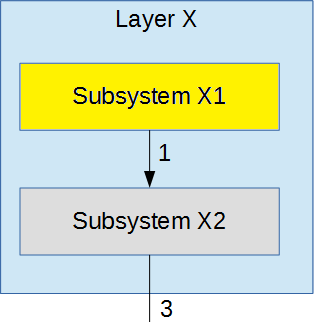
\includegraphics[width=0.60\textwidth]{images/subsystem}
 \caption{Example subsystem description diagram}
\end{figure}

\subsubsection{Subsystem Hardware}
A description of any involved hardware components for the subsystem.

\subsubsection{Subsystem Operating System}
A description of any operating systems required by the subsystem.

\subsubsection{Subsystem Software Dependencies}
A description of any software dependencies (libraries, frameworks, design software for mechanical parts or circuits, etc) required by the subsystem.

\subsubsection{Subsystem Programming Languages}
A description of any programming languages used by the subsystem.

\subsubsection{Subsystem Data Structures}
A description of any classes or other data structures that are worth discussing for the subsystem. For example, data being transmitted from a microcontroller to a PC via USB should be first be assembled into packets. What is the structure of the packets?

\subsubsection{Subsystem Data Processing}
A description of any algorithms or processing strategies that are worth discussing for the subsystem. If you are implementing a well-known algorithm, list it. If it is something unique to this project, discuss it in greater detail.



\newpage

%%% References
\bibliographystyle{plain}
\bibliographystyle{reference/IEEEtran_custom}
\bibliography{reference/refs}{}

\end{document}